\documentclass[12pt]{scrartcl}


\usepackage{epsfig,amssymb}

\usepackage{xcolor}
\usepackage{graphicx}
\usepackage{epstopdf}
\usepackage{multirow}
\usepackage{float}

\definecolor{darkred}{rgb}{0.5,0,0}
\definecolor{darkgreen}{rgb}{0,0.5,0}
\usepackage[pdfusetitle]{hyperref}
\hypersetup{
  letterpaper,
  colorlinks,
  linkcolor=red,
  citecolor=darkgreen,
  menucolor=darkred,
  urlcolor=blue,
  pdfpagemode=none,
}

\usepackage{fullpage}
\usepackage{tikz}
\pagestyle{empty} %
%obsolete: \usepackage{subfigure}
%use: 
\usepackage{subcaption}

\definecolor{MyDarkBlue}{rgb}{0,0.08,0.45}
\definecolor{MyDarkRed}{rgb}{0.45,0.08,0}
\definecolor{MyDarkGreen}{rgb}{0.08,0.45,0.08}

\definecolor{mintedBackground}{rgb}{0.95,0.95,0.95}
\definecolor{mintedInlineBackground}{rgb}{.90,.90,1}

\usepackage[newfloat=true]{minted}

\setminted{mathescape,
           linenos,
           autogobble,
           frame=none,
           framesep=2mm,
           framerule=0.4pt,
           %label=foo,
           xleftmargin=2em,
           xrightmargin=0em,
           %startinline=true,  %PHP only, allow it to omit the PHP Tags *** with this option, variables using dollar sign in comments are treated as latex math
           numbersep=10pt, %gap between line numbers and start of line
           style=default} %syntax highlighting style, default is "default"

\setmintedinline{bgcolor={mintedBackground}}
%doesn't work with the above workaround:
\setminted{bgcolor={mintedBackground}}
\setminted[text]{bgcolor={mintedBackground},linenos=false,autogobble,xleftmargin=1em}
%\setminted[php]{bgcolor=mintedBackgroundPHP} %startinline=True}
\SetupFloatingEnvironment{listing}{name=Code Sample}
\SetupFloatingEnvironment{listing}{listname=List of Code Samples}

\setlength{\parindent}{0pt} %
\setlength{\parskip}{.25cm}
\newcommand{\comment}[1]{}

\usepackage{amsmath}
\usepackage{algorithm2e}
\SetKwInOut{Input}{input}
\SetKwInOut{Output}{output}
%NOTE: you can embed algorithms in solutions, but they cannot be floating objects; use [H] to make them non-floats

\usepackage{lastpage}

%\usepackage{titling}
\usepackage{fancyhdr}
\renewcommand*{\titlepagestyle}{fancy}
\pagestyle{fancy}
%\fancyhf{}
%\rhead{Computer Science I}
%\lhead{Guides and tutorials}
\renewcommand{\headrulewidth}{0.0pt}
\renewcommand{\footrulewidth}{0.4pt}
\lfoot{\Title\ -- Computer Science I}
\cfoot{~}
\rfoot{\thepage\ / \pageref*{LastPage}}


\makeatletter
\title{Hack 7.0}\let\Title\@title
\subtitle{Lists \& Arrays \\
Computer Science I -- Java\\
{\small
\vskip1cm
Department of Computer Science \& Engineering \\
University of Nebraska--Lincoln}
\vskip-1cm}
%\author{Dr.\ Chris Bourke}
\date{~}
\makeatother

\begin{document}

\maketitle

\hrule

\section*{Introduction}

Hack session activities are small weekly programming assignments intended
to get you started on full programming assignments.  Collaboration is allowed
and, in fact, \emph{highly encouraged}.  You may start on the activity before
your hack session, but during the hack session you must either be actively 
working on this activity or \emph{helping others} work on the activity.
You are graded using the same rubric as assignments so documentation, style, 
design and correctness are all important.

%\subsection*{Rubric}
%\begin{table}[H]
%\begin{tabular}{ll}
%Category       & Point Value \\
%Style          & 2           \\
%Documentation  & 2           \\
%Design         & 5           \\
%Correctness    & 16          \\
%\textbf{Total} & \textbf{25}
%\end{tabular}
%\end{table}



\section*{Exercises}

To get more practice working with Java \mintinline{java}{List}s, you 
will write several methods that involve operations on \mintinline{java}{List}
of integers. In particular, implement the following.

\begin{enumerate}

  \item Write a method that, given a \mintinline{java}{List} of integers
  and an integer $x$ determines if it contains $x$ anywhere within the 
  \mintinline{java}{List}.  It should return \mintinline{java}{true} if it 
  does, \mintinline{java}{false} otherwise.
  
  \mintinline{java}{public static boolean contains(List<Integer> list, int x)}

  \item Write a method that, given a \mintinline{java}{List} of integers
  and an integer $x$ determines if it contains $x$ within the range of 
  the two provided indices $i, j $ (inclusive of both indices).
  It should return \mintinline{java}{true} if it 
  does, \mintinline{java}{false} otherwise.

  
  \mintinline{java}{public static boolean containsWithin(List<Integer> list, int x, int i, int j)}
  
  \item Write a method that, given a \mintinline{java}{List} of integers, 
  and a ``new size'' creates a new deep copy of the \mintinline{java}{List}.  
  However, instead of its original size, the size of the new 
  \mintinline{java}{List} should be the new size.  If the new
  size is less than the old size, only the first \mintinline{java}{newSize} 
  elements should be copied over.  If the new size is greater than the original
  size, then the new \mintinline{java}{List} should be padded out with zeros.
  
  \mintinline{java}{public static List<Integer> paddedCopy(List<Integer> list, int newSize)}

  \item Write a method that, given a \mintinline{java}{List} of integers 
  reverses the elements in the \mintinline{java}{List}.  For example, if 
  the original \mintinline{java}{List} was \mintinline{java}{[10, 15, 5, 25, 0]} 
  the new array should be 
  \mintinline{java}{[0, 25, 5, 15, 10]}.
  
  \mintinline{java}{public static void reverse(List<Integer> list)}

  \item Write a similar method that creates and returns a new, deep copy of 
  the given \mintinline{java}{List} of integers but with its elements in reverse order. 
  
  \mintinline{java}{public static List<Integer> reverseCopy(List<Integer> list)}

\end{enumerate}

\subsection*{Image Manipulation}

You'll get more practice with 2-dimensional arrays by writing several
methods to manipulate images.  In Java, you typically use a built-in
representation of an image, but we've adapted this class and instead
represent an image as a 2-dimensional array of \mintinline{java}{RGB}
``pixels'' (you've worked with this class in previous labs and hacks).  
We've written a few helper methods to load and save images to a variety 
of image file formats (jpg, bmp, gif, png, among others).  

You can manipulate individual pixels as you would any array element.  
For example:

\begin{figure}[H]
\begin{minted}{java}
RGB image[][] = ...;
RGB tempPixel = image[0][0];
...
image[i][j] = tempPixel;
\end{minted} 
\end{figure}

An image is represented by an $h \times w$ (height by width) 2D array
of these image can be represented as a two dimensional
array of these \mintinline{java}{RGB} elements.  

We've provided a library of methods to load and save a file (you'll need to 
RTM) and specified several method signatures for methods you need to
implement.  
\begin{itemize}
  \item \mintinline{c}{copyImage()} should produce a deep copy of the given
  image.
  \item \mintinline{c}{flipHorizontal()} should flip the image horizontally
  as depicted in Figure \ref{image:pointersHFlip}.
  
  \begin{figure}[h]  
  \centering
  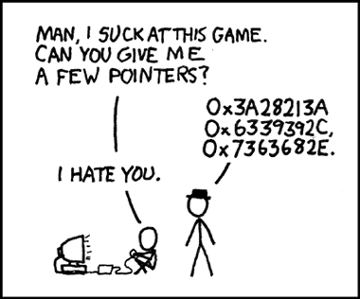
\includegraphics[scale=.50]{hack7.0-files/pointers.png}
  \caption{Original Image}
  \end{figure}
  \begin{figure}[h]  
  \centering
  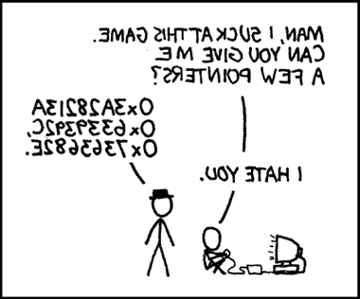
\includegraphics[scale=.50]{hack7.0-files/pointersHFlip}
  \caption{Flipped Horizontally}
  \label{image:pointersHFlip}
  \end{figure}
  \item \mintinline{c}{flipVertical()} should flip the image vertically as
  depicted in Figure \ref{image:pointersVFlip}.
  \begin{figure}[h]  
  \centering
  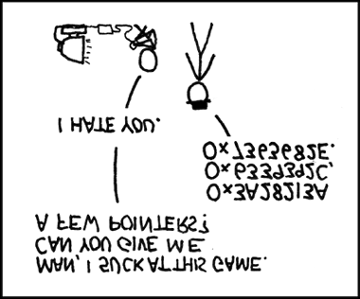
\includegraphics[scale=.50]{hack7.0-files/pointersVFlip}
  \caption{Flipped Vertically}
  \label{image:pointersVFlip}
  \end{figure}
  \item \mintinline{c}{rotateClockwise()} should produce a new image that
  is rotated 90 degrees clockwise.  This function must produce a new image
  because an $h \times w$ sized image that has been rotated will be a 
  $w \times h$ image.  This operation is depicted in Figure \ref{image:pointersRotated}.
  \begin{figure}[h]  
  \centering
  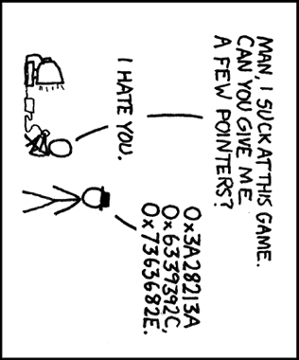
\includegraphics[scale=.50]{hack7.0-files/pointersRotated}
  \caption{Rotated Clockwise}
  \label{image:pointersRotated}
  \end{figure}
\end{itemize}  

\section*{Instructions}

\begin{itemize}

  \item For the warm-up, place all your methods with documentation in a java
  source file named \mintinline{text}{ListUtils.java} 
    
  \item In addition, you'll want to create a main test driver program 
  that demonstrates at least 3 cases per function to verify their output.  
  You need not hand in this test file, however.
  
  \item For the Image Manipulation section, we have provided starter code 
  in two source files: \mintinline{text}{ImageUtils.java} and 
  \mintinline{text}{ImageDriver.java}.  The first source file contains
  the starter code for the methods you must write.  The driver file 
  contains a main that you can use to test your program on an image of
  your choice.
  
  \item You should test all your functions with an image (load it, manipulate
  it and save it) of your choice.
  
  \item As a first step, you should add documentation to all your functions.
  Use this as an opportunity to discuss how the functions should work and
  to \emph{whiteboard} your designs and solutions with other students.
  
  \item You are encouraged to collaborate any number of students 
  before, during, and after your scheduled hack session.  

  \item You may (in fact are encouraged) to define any additional
  ``helper'' methods that may help you.
  
  \item Include the name(s) of everyone who worked together on
  this activity in your source file's header.

  \item Turn in all of your files via webhandin, making sure that 
  it runs and executes correctly in the webgrader.  Each individual 
  student will need to hand in their own copy and will receive 
  their own individual grade.
\end{itemize}  


\end{document}
